\documentclass[abstract=true]{scrartcl}
\subject{Beeldbewerken \\ Assignment 3: ``Finding Waldo''}
\title{}
\author{Joris Stork, Lucas Swartsenburg}
\usepackage{graphicx,amsmath,subfig}
\addtolength{\parskip}{\baselineskip}
\begin{document}
\maketitle


\section{Histogram intersection}

    \subsection{Colour histogram exercise}

        \subsubsection{``What type of array do you need to store a colour
            histogram?''}

            One needs an array (of floats) of dimension $n$ where $n$ is the
            number of components in the colour model. In this case, a three
            dimensional array. The indexes in each dimension together index the
            bins of a three dimensional histogram. The values in the ultimately
            indexed elements represent the numbers of pixels in the image that
            display the colour corresponding to that bin. 

    \subsection{Histogram intersection exercise}

\begin{figure}
  \centering
  \subfloat[air1]{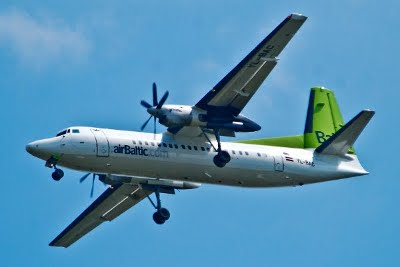
\includegraphics[width=0.3\textwidth]{../images/database/air1}}                
  \subfloat[air2]{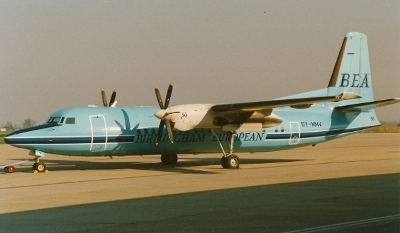
\includegraphics[width=0.3\textwidth]{../images/database/air2}}
  \subfloat[air3]{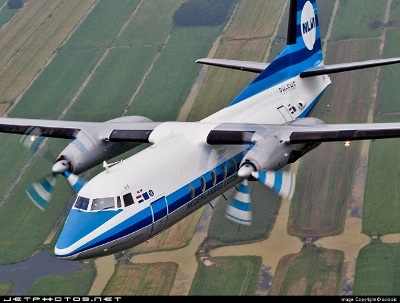
\includegraphics[width=0.3\textwidth]{../images/database/air3}}\\
  \subfloat[air4]{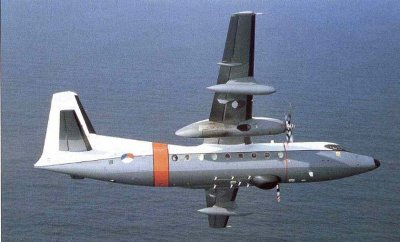
\includegraphics[width=0.3\textwidth]{../images/database/air4}}                
  \subfloat[bre1]{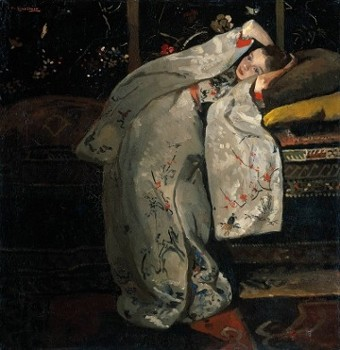
\includegraphics[width=0.3\textwidth]{../images/database/bre1}}
  \subfloat[bre2]{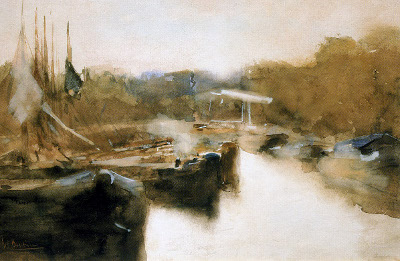
\includegraphics[width=0.3\textwidth]{../images/database/bre2}}\\
  \subfloat[leds]{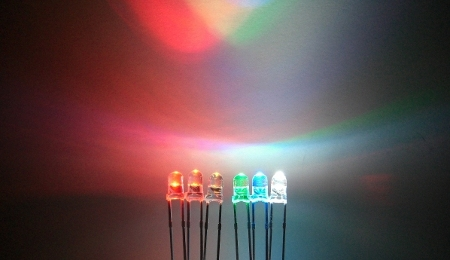
\includegraphics[width=0.3\textwidth]{../images/database/leds}}                
  \subfloat[fire]{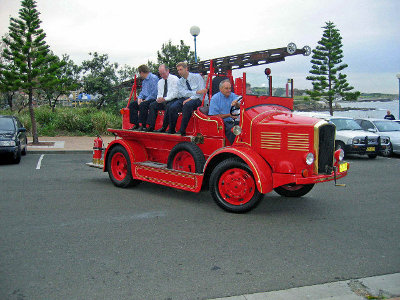
\includegraphics[width=0.3\textwidth]{../images/database/fire}}
  \subfloat[lbug]{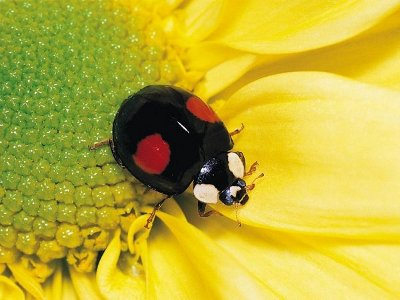
\includegraphics[width=0.3\textwidth]{../images/database/lbug}}\\
  \subfloat[star]{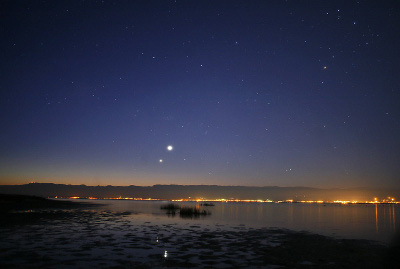
\includegraphics[width=0.3\textwidth]{../images/database/star}}
  \caption{"database" images}
\end{figure}

\begin{figure}
  \centering
  \subfloat[airb]{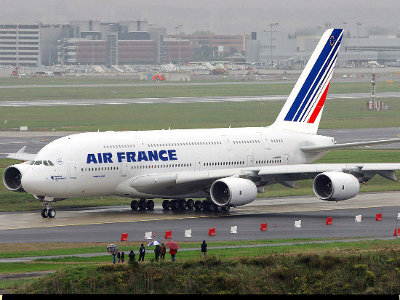
\includegraphics[width=0.3\textwidth]{../images/external/airb}}
  \subfloat[rcar]{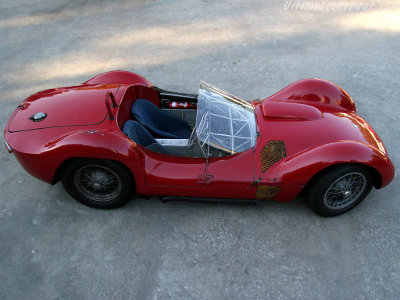
\includegraphics[width=0.3\textwidth]{../images/external/rcar}}
  \subfloat[flag]{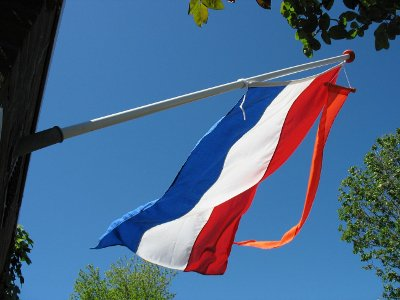
\includegraphics[width=0.3\textwidth]{../images/external/flag}}\\
  \caption{"external" images}
\end{figure}

\begin{table}
    \begin{tabular}{l l | *{10}{c}}

              &Model&air2&bre1&air4&leds&air3&fire&star&air1&lbug&bre2\\  
        Image &     &    &    &    &    &    &    &    &    &    &    \\ 
        \hline
        air2  &     &1.00&0.20&0.06&0.11&0.13&0.14&0.07&0.05&0.05&0.24\\  
        bre1  &     &0.25&1.00&0.07&0.30&0.25&0.14&0.30&0.05&0.10&0.32\\  
        air4  &     &0.06&0.06&1.00&0.21&0.22&0.24&0.16&0.12&0.02&0.08\\  
        leds  &     &0.14&0.30&0.25&1.00&0.25&0.31&0.27&0.17&0.09&0.17\\  
        air3  &     &0.17&0.26&0.28&0.26&1.00&0.44&0.22&0.13&0.06&0.26\\  
        fire  &     &0.18&0.14&0.30&0.32&0.43&1.00&0.19&0.15&0.07&0.22\\  
        star  &     &0.09&0.27&0.17&0.25&0.20&0.17&1.00&0.09&0.08&0.16\\  
        air1  &     &0.06&0.05&0.14&0.15&0.12&0.14&0.09&1.00&0.02&0.05\\  
        lbug  &     &0.06&0.10&0.02&0.09&0.06&0.07&0.09&0.03&1.00&0.13\\  
        bre2  &     &0.27&0.28&0.09&0.15&0.22&0.19&0.16&0.04&0.11&1.00

    \end{tabular}
    \caption{RGB intersections within database}
\end{table}

\begin{table}
    \begin{tabular}{l l | *{10}{c}}

              &Model&air2&bre1&air4&leds&air3&fire&star&air1&lbug&bre2\\  
        Image &     &    &    &    &    &    &    &    &    &    &    \\  
        \hline
        airb  &     &0.26&0.28&0.20&0.27&0.42&0.37&0.20&0.09&0.07&0.36\\  
        rcar  &     &0.16&0.13&0.35&0.37&0.31&0.33&0.18&0.11&0.08&0.18\\  
        flag  &     &0.09&0.15&0.14&0.19&0.18&0.25&0.18&0.20&0.09&0.15

    \end{tabular}
    \caption{RGB intersections against external images}
\end{table}

    \subsection{Colour model exercise}

        For this exercise we have chosen the YUV colour model. We had initially
        chosen HSV, an implementation for which is embedded in our application.
        However, we chose YUV since HSV is sometimes classified as a
        sub-representation of RGB, and not as a distinct colour model.

        \subsubsection{``... what are the conversion formula's...''}
        
            The formula for RGB to YUV conversion is straightforward (source:
            Wikipedia):

            \begin{eqnarray}
                \begin{bmatrix} Y \\ U \\ V \end{bmatrix} = 
                \begin{bmatrix} 
                    0.299 & 0.587 & 0.114 \\
                    -0.14713 & -0.28886 & 0.436 \\
                    0.615 & -0.51499 & -0.10001 
                \end{bmatrix}
                \begin{bmatrix} R \\ G \\ B \end{bmatrix}
            \end{eqnarray}

        \subsubsection{Description of YUV model}

            The YUV model is a European (PAL) standard and the equivalent of the
            US (NTSC) standard, YIQ. The model was created for the broadcasting
            industries of the 20th century as a means to efficiently transmit
            colour video signals. The YUV model takes certain characteristics of
            human colour perception into account to reduce the bandwidth needed
            to transmit chrominance (as opposed to luminance) components of the
            image.

        \subsubsection{Effect of YUV model on histogram intersections}

\begin{table}
    \begin{tabular}{l l | *{10}{c}}

              &Model&air2&bre1&air4&leds&air3&fire&star&air1&lbug&bre2\\  
        Image &     &    &    &    &    &    &    &    &    &    &    \\  
        \hline
        airb  &     &0.39&0.33&0.23&0.35&0.49&0.32&0.23&0.09&0.09&0.49\\
        rcar  &     &0.12&0.13&0.60&0.37&0.22&0.49&0.21&0.15&0.07&0.20\\
        flag  &     &0.12&0.14&0.15&0.20&0.22&0.28&0.14&0.17&0.09&0.15 

    \end{tabular}
    \caption{YUV intersections against external images}
\end{table}

            A quick comparison of the intersection tables for RGB and YUV shows
            apparently non-linear differences in the way intersections are
            evaluated for these two colour models.

            For instance, the YUV model appears to better reflect the similarity
            between the fire truck and red car. One could speculate that the YUV
            model better accounts for the perceived similarity of the red
            vehicles, where perhaps the RGB model ``notices'' the difference
            between the two reds more ``literally''.

            Interestingly, the YUV model shows a significantly higher value
            between ``air4'' and the red car, than the RGB model. The YUV
            implementation would appear to lend greater weight to the similarity
            between the respective gray sea background and gray asphalt
            background.

\section{Colour back projection}

    \subsection{Colour back projection exercise}
        
        Refer to the application (menu option 3) and source code. Note that the
        number of bins can easily be adjusted within \texttt{menu()}.

        It is also worth noting that the expected location returned by our
        implementation corresponds to a sailor near the bottom of the image. His
        trouseres feature a similar colour pattern to Waldo's, but larger. This
        suggests that tweaks to the convolution kernel's size in our
        implementation should result in improved results. 

\begin{figure}
  \centering
  \subfloat[where's Waldo?]{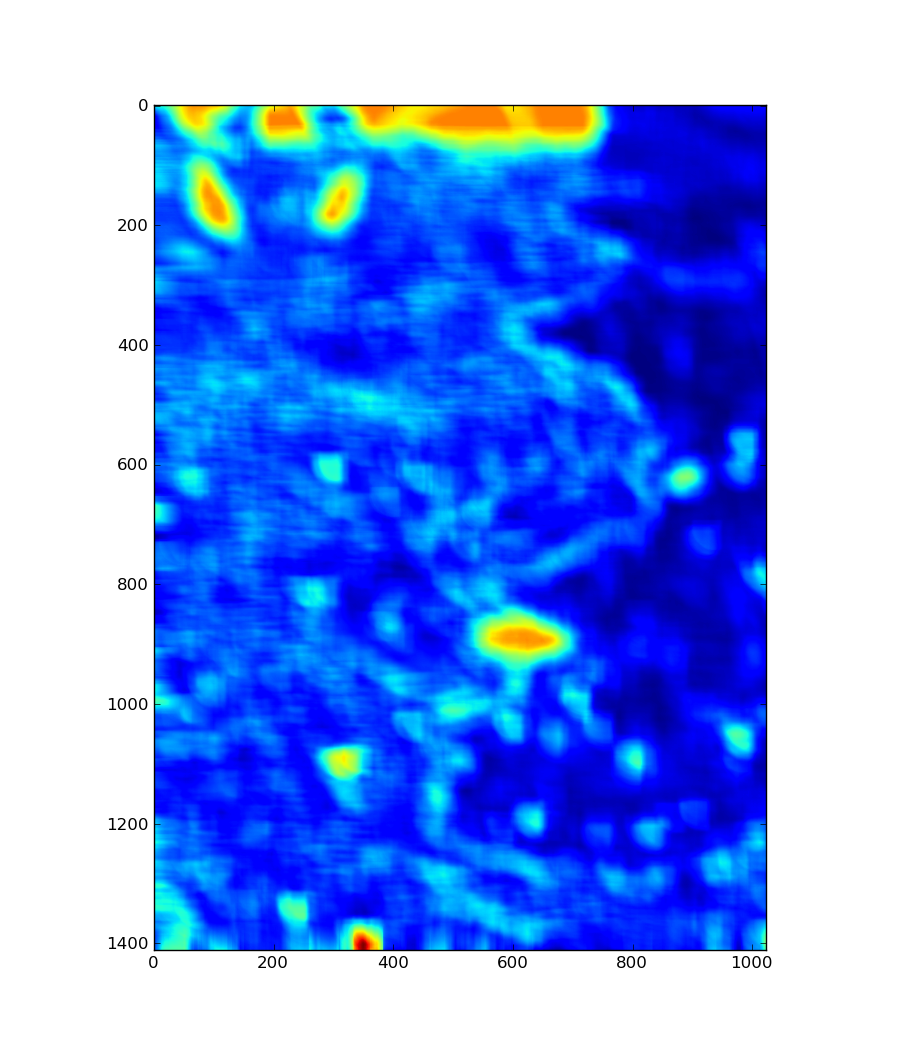
\includegraphics[width=0.75\textwidth]{../images/waldo/expected}}
  \caption{expectation heatmap: Waldo's location}
\end{figure}

\end{document}
